\documentclass[12pt]{article}
\usepackage{pgfplots, url, tikz, graphicx}
\usepackage{enumitem} % To customize enumerate
\usepackage{amssymb}
\usepackage{caption}
\usepackage{subcaption}
\usepackage{amsmath}
\usepackage{float}
\usepackage{sagetex}

\usetikzlibrary{arrows.meta, positioning}
\pgfplotsset{compat=1.18}

\title{Math HW Week 9}
\author{Duc Nguyen}
\date{\today}

\begin{document}
\maketitle
\section*{3.6}
\subsection*{\#1}
\begin{figure}[htbp] % h=here, t=top, b=bottom, p=page of floats
  \centering
  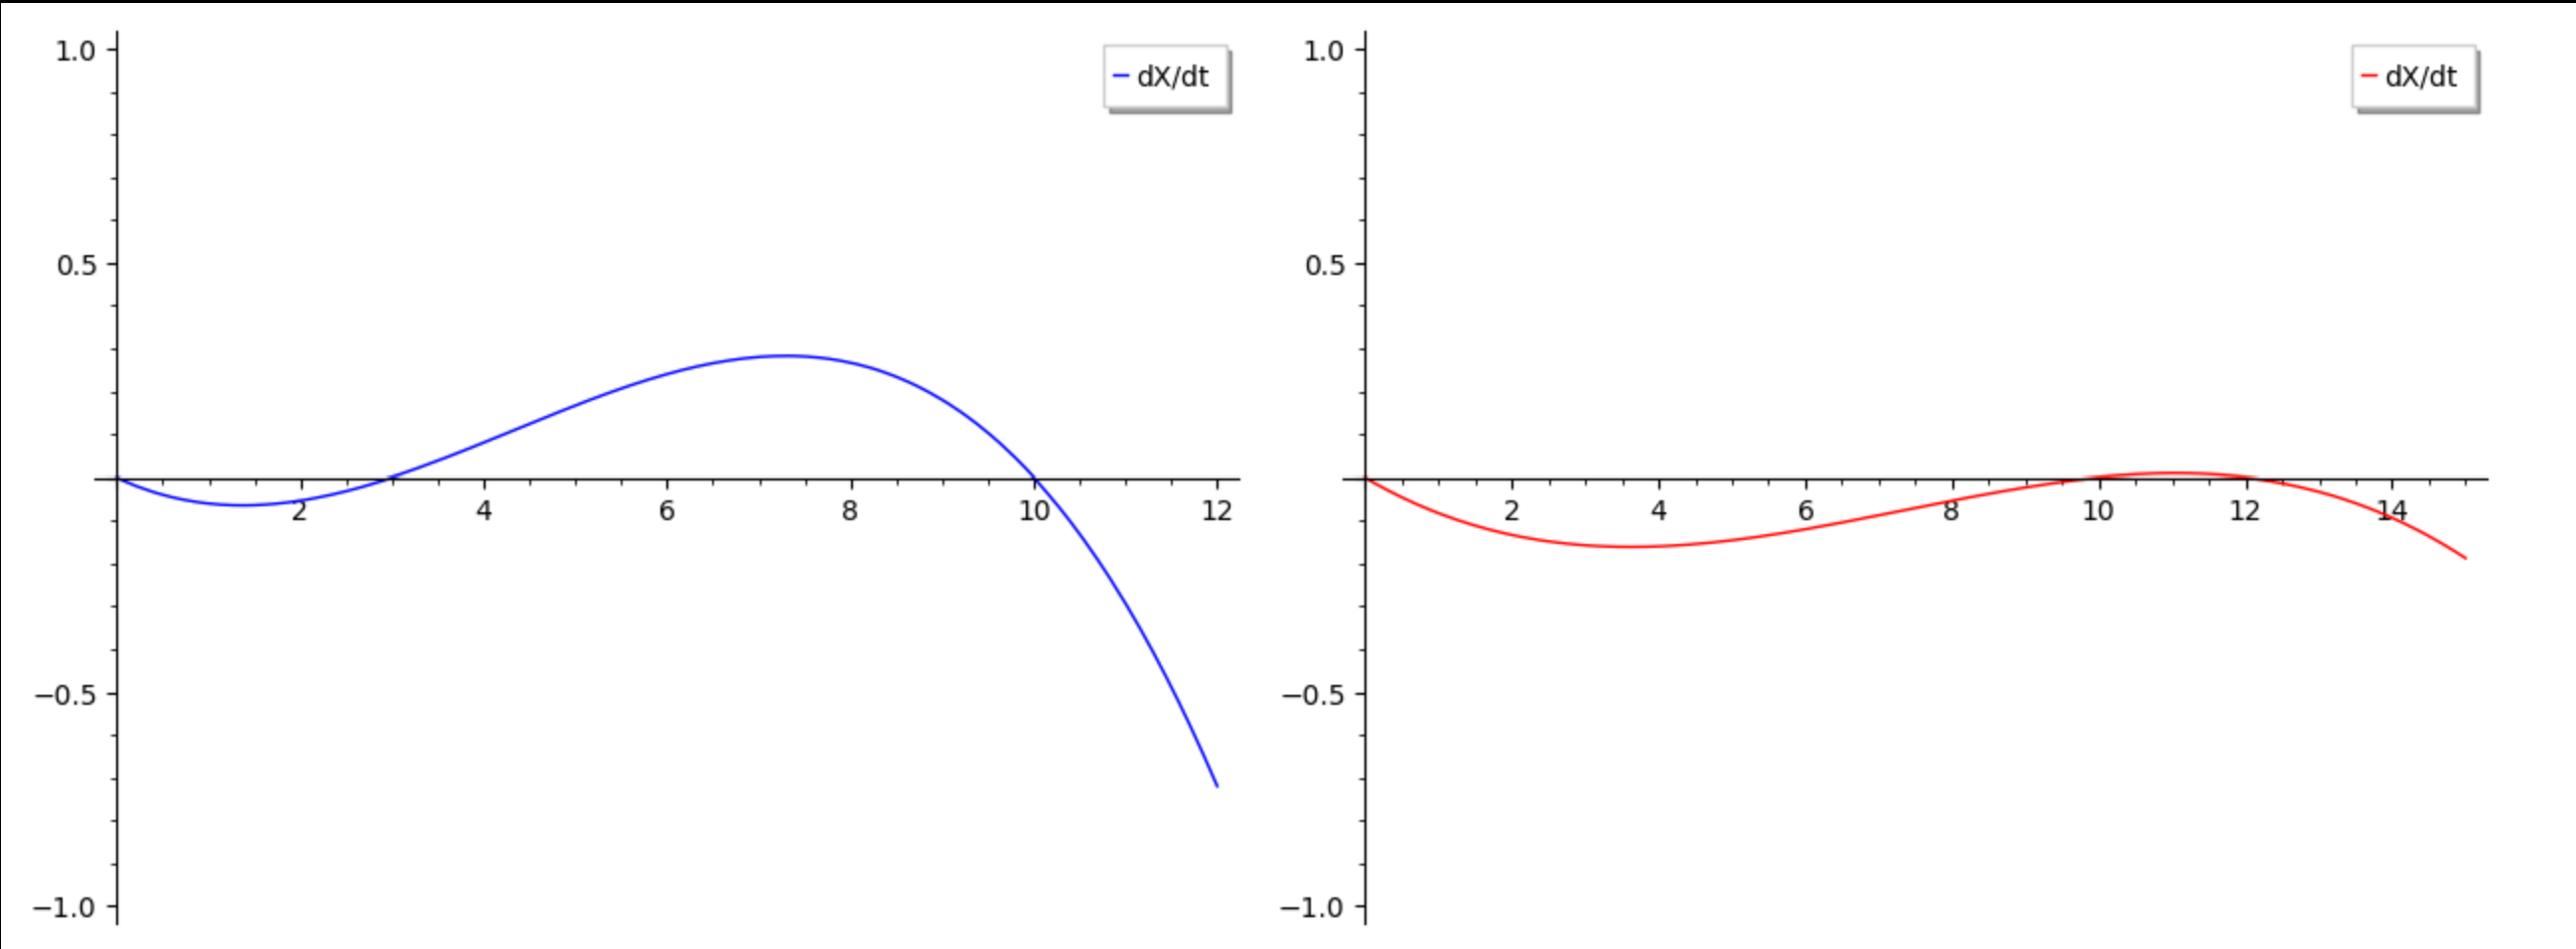
\includegraphics[width=0.6\textwidth]{hw9.png}
\end{figure}

\subsection*{\#2}
At a = 600, It still stable because k doesn't exceed a yet. But at a = 900, the equilibrium start to transition from a to k and gets unstable. At a = 1200, the equilibrium is transfer to a and k is no longer stable.

\subsection*{\#3}
Yes because in a saddle-node bifurcation, the pair of equilibria always consists of one stable equilibrium and one unstable equilibrium

\subsection*{\#4}
There're 3 cases: 

Case 1: Low k or Low r

The over-under method shows $X' > 0$ below, but $X' < 0$ above $=>$ stable equilibrium. This means that the predators suppress budworm, hence population remains low

Case 2: Moderate/High k and increasing r

Using the over-under method, we can find three equilibria:
Left: Stable equilibrium (refuge)
Middle: Unstable equilibrium (tipping point)
Right: Stable equilibrium (outbreak)

Between refuge and tipping point, we have:
$X' < 0 =>$ population decreases $->$ unstable
Between tipping point and outbreak, we have:
$X' > 0 =>$ population increases $->$ stable

Case 3: Very high r (after bifurcation)

Using the method, we only found one high equilibrium (outbreak), this means that system has lost control of pest population

As habitat improves, pest growth overcomes predation. The system undergoes saddle-node bifurcation: two equilibria born,with the unstable equilibrium acts as a tipping point between refuge and outbreak. Hence confirm the statenent.

\subsection*{\#5}
The higher the growth rate r, the more likely the system will undergo a saddle bifurcation.

\subsection*{\#6}
\begin{enumerate}[label=\alph*.]
    \item (k=10,r=0.1)
    There's one equilibrium at low. It's stable
    \item (k=25,r=0.6)
    There's 3 equilibria: one stable at low, one unstable at medium, and one stable at high. 
    \item (k=20,r=0.4)
    Also the same to previous case, all 3 equilibria: one stable at low, one unstable at medium, and one stable at high.
\end{enumerate}

\section*{Further Exercises 3.6}
\subsection*{\#1}
They make sense biologically in both case, stable when $A < K$, unstable when $A > K$. Therefore to make it stable, we need to keep $0 < A < K$. (As 0 means extinction)
\subsection*{\#2}
\begin{enumerate}[label=\alph*.]
    \item Around 0.4
    \item Around 5.5 to 6
    \item Around 7
    \item At 0.8, there's more turbidity because it also reach the upper bound around 5.5 to 6
    \item It has to be under 0.5
    \item Our lake has become cloudy due to too many nutrients, mostly from fertilizer runoff. Even though we've tried reducing nutrients a bit, the water didn't get clearer. That's because the lake needs a bigger push to flip back to its natural clear state. To really fix the problem, we need to cut nutrient input significantly — likely by reducing fertilizer use from gardens and lawns. This might feel like a big change, but it's necessary to bring back the clean, healthy water that we all want to enjoy.
\end{enumerate}
\subsection*{\#3}
\begin{enumerate}[label=\alph*.]
    \item There're 2 saddle-node bifurcation. At r = 15, the lower stable and middle stable branch merge. At r = 30, the upper stable and middle stable branch merge.
    \item 2 stable points
    \item X will increases, coordinate with the muscle tone
    \item At r = 22, both stable branches are present. Depends on the initial condition, X will either converge to the lower stable branch (low) or the upper stable branch (high).
\end{enumerate}
\subsection*{\#4}
\begin{enumerate}[label=\alph*.]
    \item There're all 3 saddle-node bifurcation at r = 35,55,75. 
    \item There're 3 equilibria: 2 stable one at $x < 0.4$ and 1 unstable one at $x > 0.4$
    \item If r increases past 55, the bass population drops. But if r decreases past 35, the population recovers. It shows that the population will collapse until more carbon input are reduced
    \item Increase r to above 75, because we're on a low stable branch, if we increase r, the bass population will increase to the upper stable branch. The population will then stabilize until r went down to 55 for some reason.
\end{enumerate}

\end{document}